\begin{section}{Results}
\label{sec:lmoeda-mgmof}

\begin{subsection}{Initial Force Field and Cluster Model Analysis}

Originally, we attempted to fit Mg parameters on the basis of a small, 6 heavy
atom cluster (`\mgmof-small', see \cref{fig:lmoeda-small_fit} for
chemical structure), which we felt would be
representative of the Mg environment in \mgmof. Using the functional forms
discussed in \cref{sec:lmoeda-methods}, force field parameters were fit to
reproduce \lmoeda-\pbeod energies for a variety of \co/\mgmof-small
interactions, with results shown in \cref{fig:lmoeda-small_fit}.
Though select interaction energies disagree by several \kjmol{} between
\lmoeda-\pbeod and the force field energies, overall the agreement is
reasonable, and the force field correctly reproduces trends in the interaction
energies without significant systematic error. 


    %%%%%%%%%%%% Small Energies %%%%%%%%%%%%%%%
    \begin{figure}
    \centering
    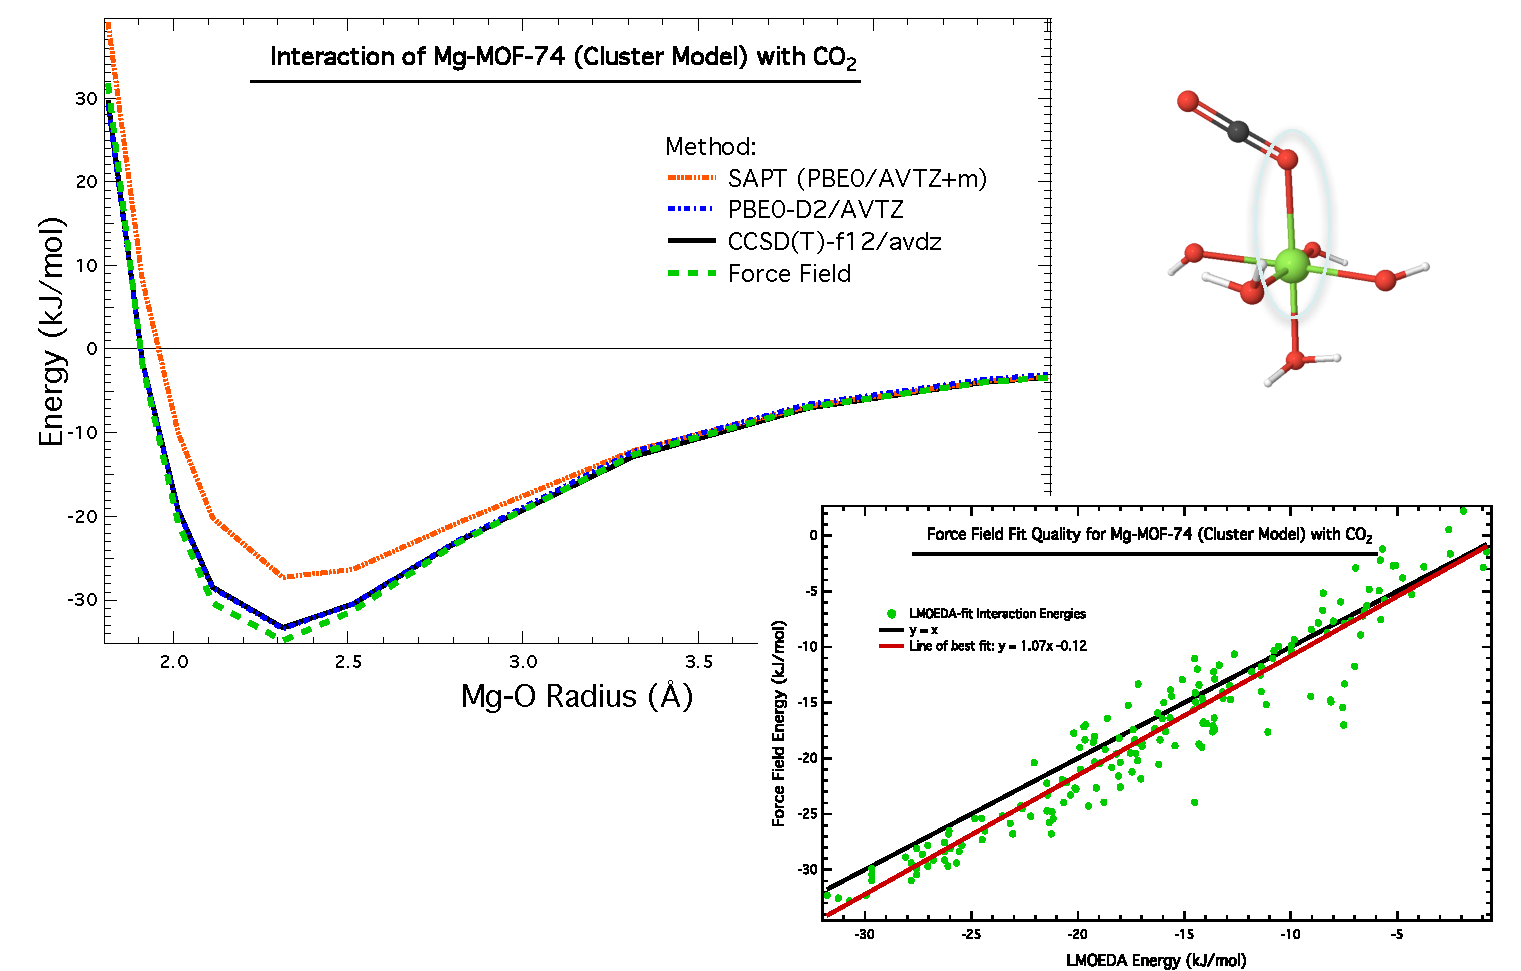
\includegraphics[width=1.0\textwidth]{lmoeda/small_energies.pdf}
    \caption[Force field fitting quality for the \mgmof-small cluster]
{Force field fitting quality for the \mgmof-small cluster. (Top left) Various
electronic structure benchmarks for \mgmof-small along with the classical
potential. Each \dftsapt (orange dot-dashed), \pbeod (blue dot-dashed), \ccsdtf (black
solid), and the \lmoeda-based force field (green dashed) are shown as a
function of the \ch{Mg-O} interatomic distance (non-bonding pair highlighted
at top right). (Bottom right) Force field fit quality, as benchmarked against
\lmoeda-\pbeod, for a semi-random set of dimer configurations of the
\mgmof-small cluster model interacting with \co. The black line
establishes the $y=x$ benchmark, and the red line represents the line of best
fit.
            }
    \label{fig:lmoeda-small_fit}
    \end{figure}
    %%%%%%%%%%%% Small Energies %%%%%%%%%%%%%%%


Based on the agreement between
\pbeod and the force field, as well as between \pbeod and \ccsdtf, we expected
to obtain good \co adsorption isotherm predictions for the \mgmof system
itself. By contrast, our computed isotherm substantially underpredicts the
experimental adsorption at low pressures, where Mg--\co interactions are known
to dominate. This underprediction strongly suggests that we had originally
underestimated the magnitude of the Mg--\co binding, a result which we were
then able to attribute to our choice of cluster model (vida infra).

    %%%%%%%%%%%% Clusters %%%%%%%%%%%%%%%%%%%%%
    \begin{figure}
    \centering
    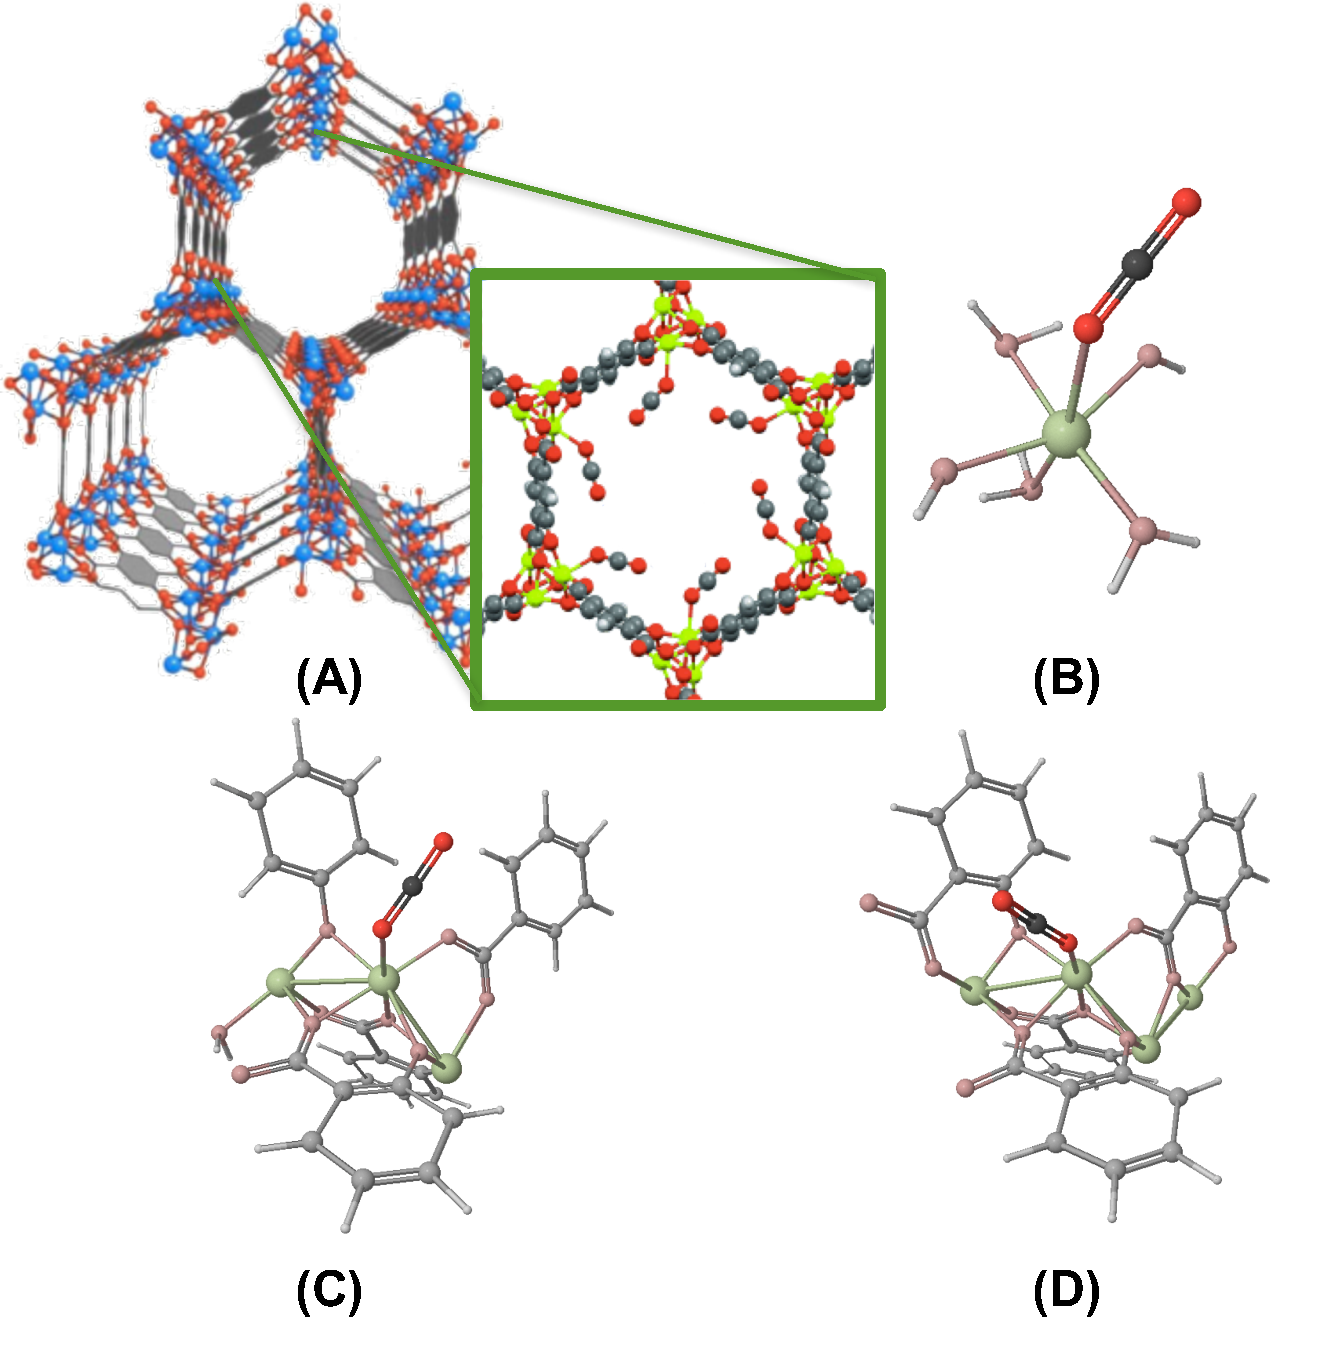
\includegraphics[width=0.8\textwidth]{lmoeda/clusters.pdf}
    %
    \renewcommand\arraystretch{1.1}
    \begin{tabular}{@{}lccc@{}}
    \hline
    \toprule
    
    Model & \co Binding Energy & Mg--O Interatomic Distance & Mg--O--C Tilt Angle  \\ 
          & (kJ/mol) & (\AA) & ($^{\circ}$) \\ 
    
    \midrule
    \textbf{A}\cite{Valenzano2010} & \textbf{-41.5} & \textbf{2.31} &
\textbf{129}     \\
    B                           & -23.3 & 2.31 & 122     \\
    C                           & -31.4 & 2.28 & 123     \\
    D                           & -41.7 & 2.20  & 149     \\


    %
    \bottomrule
    \hline
    \end{tabular}

    \caption[Model clusters for \mgmof]
{ Various structures and cluster models for \mgmof interacting with \co. 
(A) Full periodic \mgmof structure with inset showing adsorbed \co positions. 
(B) \mgmof-small cluster, containing 6 heavy atoms (not including \co). 
(C) \citeauthor{Yu2012c} cluster model for \mgmof, denoted in text as \mgmof-Yu.
(D) \citeauthor{Dzubak2012} cluster model for \mgmof, denoted in text as
\mgmof-Dzubak.
All cluster models as shown with optimized \co positions, and bond lengths and
angles for adsorbed \co are given in the bottom table. Data for (A) was taken
from \citeauthor{Valenzano2010} using a B3LYP-D level of theory,\cite{Valenzano2010}
whereas data for (B-D) was computed in this work using \pbeod. Finally, note
that the binding energy for (A) includes framework geometry relaxation effects,
whereas (B-D) were computed using semi-rigid cluster geometries and only optimizing
the \co position and exposed \ch{MgO5} pocket.
            }
    \label{fig:lmoeda-clusters}
    \end{figure}
    %%%%%%%%%%%% Clusters %%%%%%%%%%%%%%%%%%%%%

Cluster models for the M-MOF-74 series have been investigated by several
groups, and it has been found in general that computed binding energies are
sensitive both to the size of the cluster model as well as the treatment of
geometry relaxation effects.\cite{Verma2013,Valenzano2011} Consequently, we
calculated the \co binding energies and geometries of both our original
\mgmof-small cluster as well as for two larger clusters developed in
\citens{Yu2012c,Dzubak2012}. These latter two clusters, respectively denoted
\mgmof-Yu and \mgmof-Dzubak, are the same size (each with 60 atoms), but have
distinct stoichiometries and geometries.
To test the influence of model
cluster on the \co binding energy/geometry, we performed two sets of
optimizations of the \mgmof-Yu and \mgmof-Dzubak clusters: one in which only
the \co position was optimized, and one in which the exposed \ch{MgO5} pocket
was additionally relaxed. Binding geometries were relatively insensitive to
the geometry relaxation, though binding energies varied by \kjmol{2-5}, in
agreement with other studies that have tested geometry
relaxation effects.\cite{Verma2013} Results for the \ch{CO2 + MgO5} relaxation are shown in
\cref{fig:lmoeda-clusters}. 

Of the three studied cluster models, both \mgmof-small and \mgmof-Yu correctly
reproduce the \ch{Mg-O} interatomic distance and \ch{Mg-O-C} tilt angle. These
geometrical parameters arise primarily from electrostatic interactions between
\co and the \ch{MgO5} pocket,\cite{Valenzano2010} 
suggesting that both of these models capture such important interaction
features. By contrast, the \mgmof-Dzubak model predicts a substantially shorter binding
distance and increased tilt angle, both in contrast to results from the
periodic system. In part, these deficiencies can be attributed to spurious
\co interactions with the exposed carbonyl capping groups in the \mgmof-Dzubak
model, as these exposed carbonyls are not present in the periodic system or the other two cluster
models. As a second distinction, a Mulliken charge analysis of the 
\mgmof-Dzubak cluster yields larger partial charges for the surrounding Mg
atoms as compared to the \mgmof-Yu model, which may help explain the increased
binding and shortened \ch{Mg-O} contact in the \mgmof-Dzubak model. 

There are also substantial differences in binding energies
between the various cluster models. Importantly, \mgmof-small severely
underbinds
\co compared to all other tested systems.
These results for the \mgmof-small cluster indicate the inadequacy of such a small 
model, and likely explain the underprediction of the \co adsorption isotherm
from above. 
The \mgmof-Dzubak model shows best energetic agreement with the periodic system. 
Nevertheless, some of the \mgmof-Dzubak binding energy arises from 
truncation effects (as described above), and the energetic agreement is thus
due (at least in part) to error cancellation. Indeed, some of the binding
energy in the periodic system arises from (attractive) long-range
interactions, and thus we should expect to see a cluster model somewhat
underpredict the binding energy. 
Primarily for its good agreement in binding geometries, and reasonable
agreement in binding energy, 
we opt to use the \mgmof-Yu cluster model for the remainder of this work.

\end{subsection}
\begin{subsection}{Final Mg-MOF-74 {\co} Adsorption Isotherm}

Using our new \mgmof-Yu cluster model, we next attempted to refit
force field paramters for Mg. As discussed earlier, and
because of the size of this new cluster (60 atoms), \lmoeda-\pbeod
calculations became cost prohibitive in all but the smallest VDZ basis set, and
thus could only be carried out for a limited set of points. Starting from the minimum energy configuration
shown in \cref{fig:lmoeda-clusters}, we fit Mg parameters to a 12-point scan along the
Mg-O bond vector, with fit results shown in  
\cref{fig:lmoeda-xlarge_fit}. Interestingly, though the functional form used
in this fit was sufficient to accurately paramterize the interaction energies
in the \mgmof-small cluster, the same force field methodology proved
unsuccessful in paramterizing \mgmof-Yu--\co interactions. We knew at the time that
this inaccuracy was probably a consequence of uncertainties in correctly
parameterizing the Mg short-range exponent. (See \cref{ch:isaff} for a full
discussion of new methods for parameterizing the short-range potential.) Nevertheless, because the Slater-ISA methodology
for short-range interactions had not yet been developed, we opted instead to
fit the Mg interactions to a double exponential functional form, with each
exponent corresponding to the ionization potential for either \ch{Mg+} or
\ch{Mg^{2+}} (the two atomic environments most likely to correctly
represent the Mg cation). As shown in \cref{fig:lmoeda-xlarge_fit}, this
form could excellently reproduce the \mgmof-Yu model \pes.


    %%%%%%%%%%%% Xlarge Cluster Fitting %%%%%%%
    \begin{figure}
    \centering
    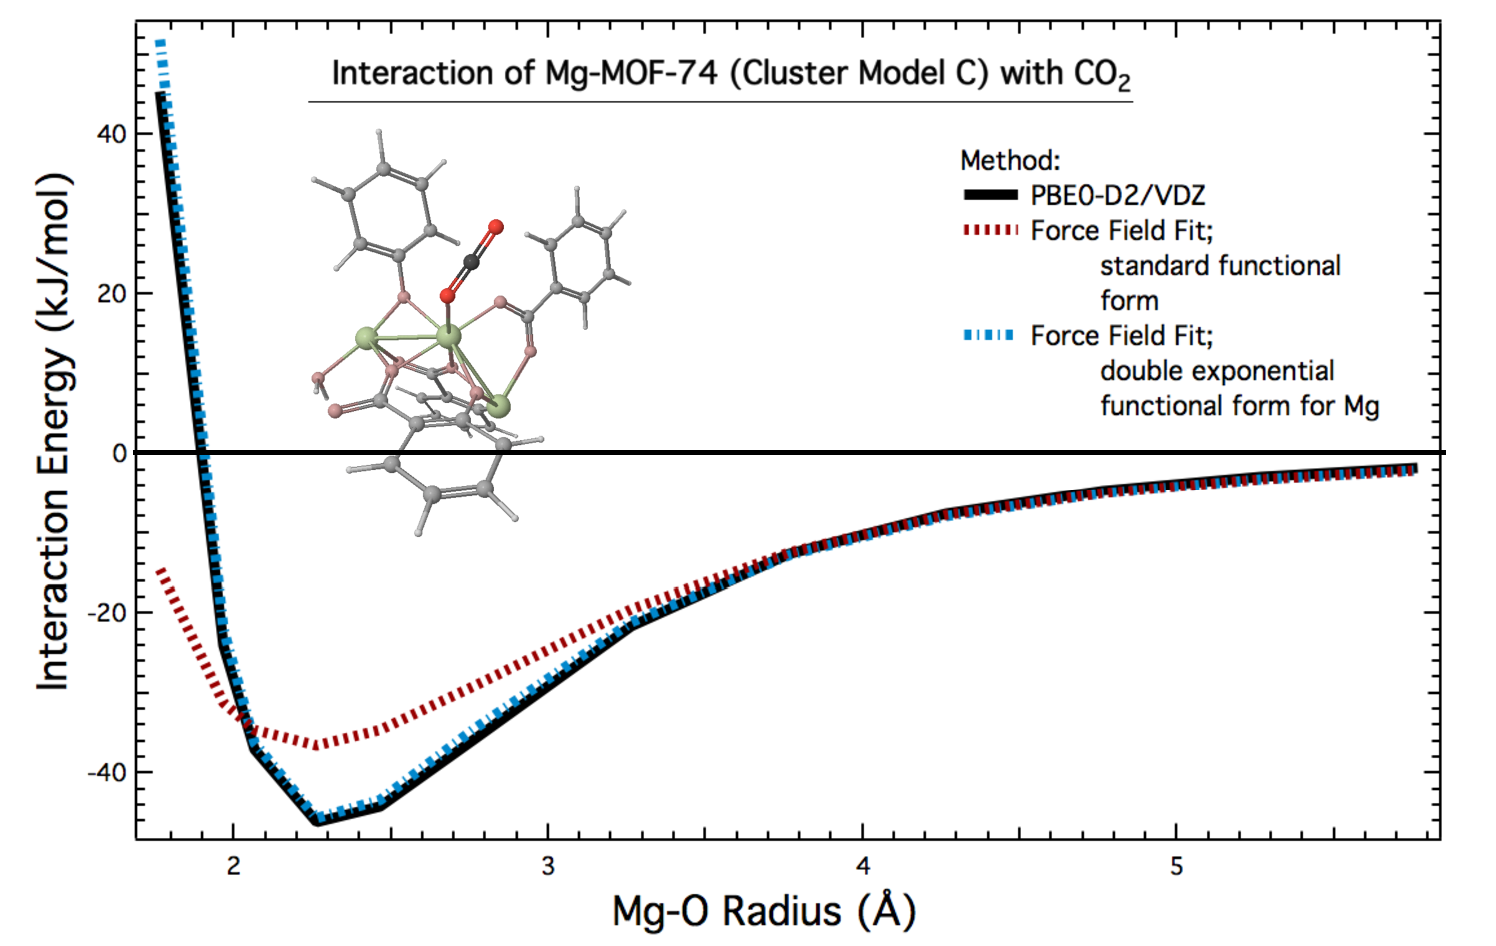
\includegraphics[width=1.0\textwidth]{lmoeda/xlarge_ff_fit.pdf}
    \caption[Force field fitting quality for \mgmof-Yu]
{Force field fitting quality for the \mgmof-Yu cluster. A \pbeod benchmark
(black solid) is displayed along with two force field fits: single-exponential
(red dashed) and double-exponential for Mg (blue dash-dotted). In either case,
a cut of the \pes is shown along the interatomic distance between the central
Mg atom and the closest-contact oxygen atom in \co.
            }
    \label{fig:lmoeda-xlarge_fit}
    \end{figure}
    %%%%%%%%%%%% Xlarge Cluster Fitting %%%%%%%


Using the double exponential functional form from above, we recomputed the
 adsorption isotherm of \co in \mgmof. Before comparing to experiment, and as
recommended by others,\cite{Haldoupis2015a} we scaled the experimental
isotherm in order to account for the pore blocking effects that are common in
the M-MOF-74 series. Using this scaled isotherm, we then obtain excellent
agreement between our model potential and experiment
(\cref{fig:lmoeda-isotherm}). Crucially, this accuracy is seen both at low-
and high-pressure ranges, indicating the accuracy of the force field in
modeling both the
strong \ch{Mg-CO2} binding as well as the weaker physisorption regime.



    %%%%%%%%%%%% MgMOF Adsorption %%%%%%%%%%%%%
    \begin{figure}
    \centering
    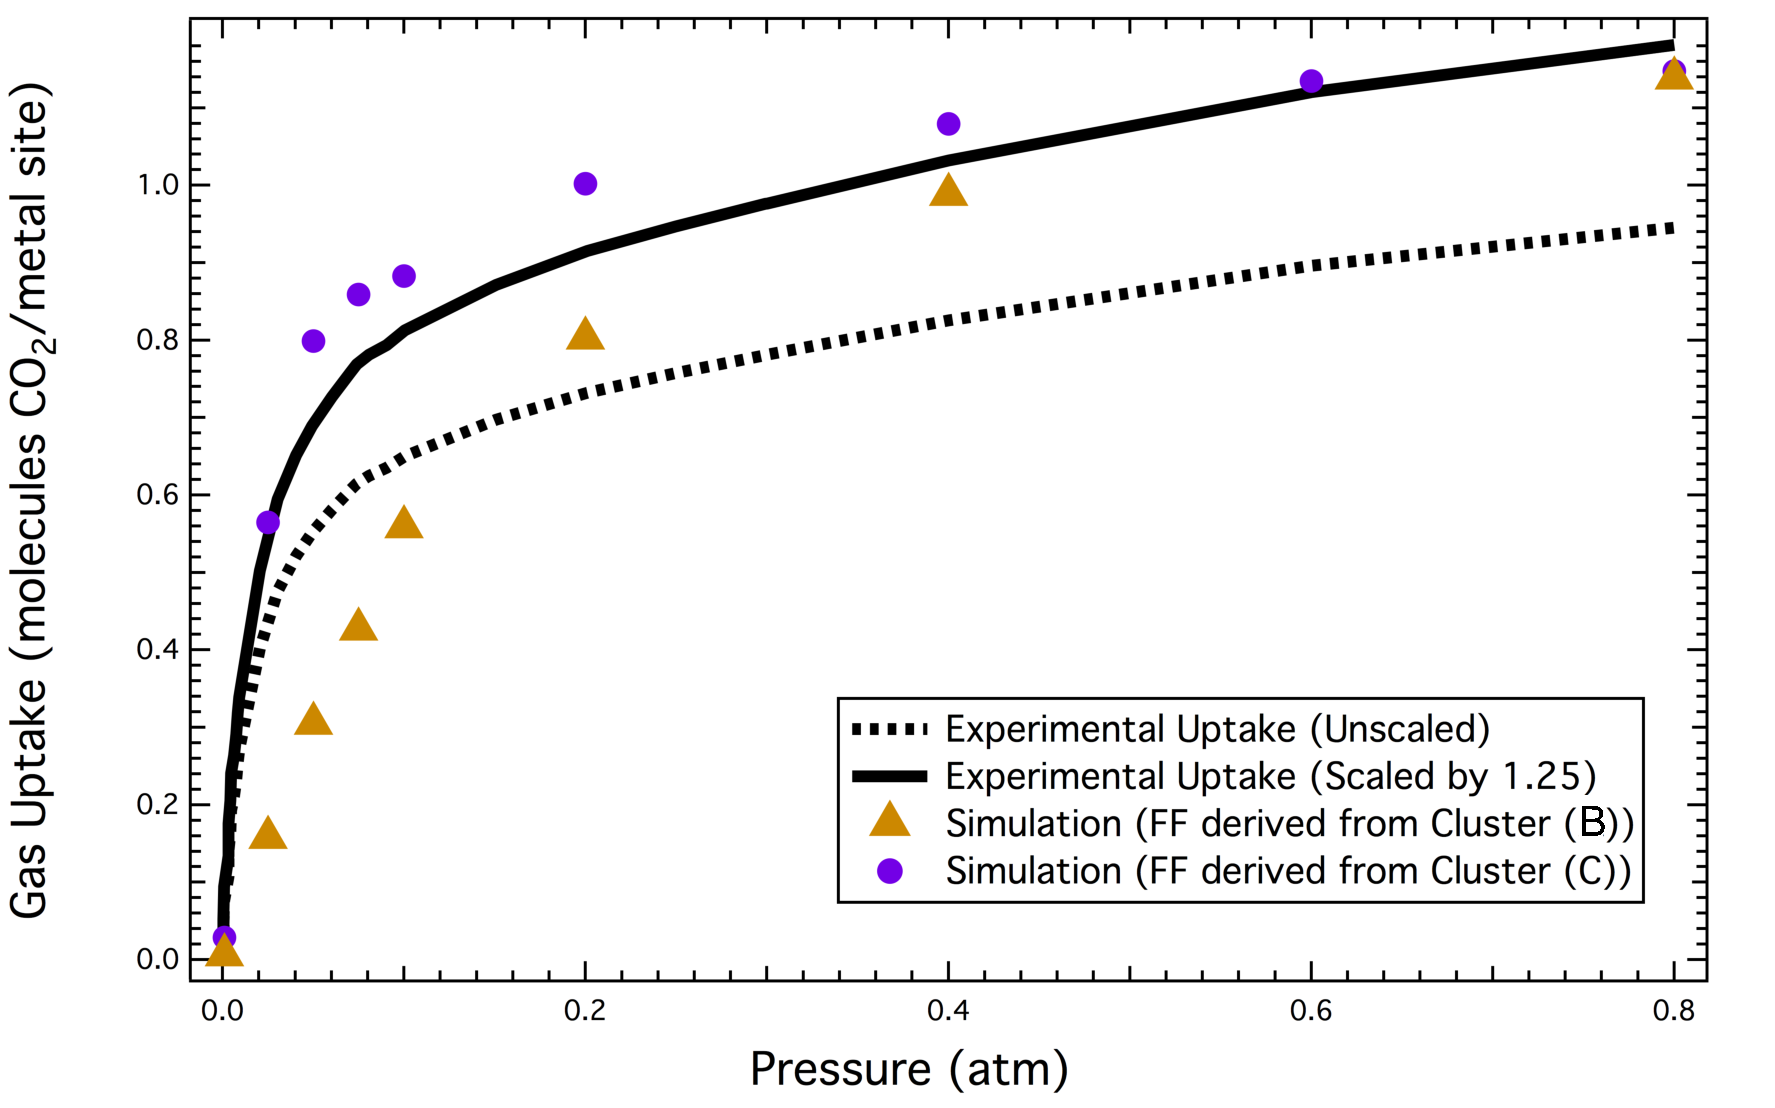
\includegraphics[width=1.0\textwidth]{lmoeda/mgmof_isotherm.pdf}
    \caption[Predicted \co Adsorption Isotherm for \mgmof]
{Predicted \co adsorption isotherm for \mgmof. Two experimental isotherms are
shown, one as directly measured by experiment (dashed line) and one scaled to
account for pore block effects (solid line). Predictions from two force fields
are also shown, where Mg parameters for each force field were fit either to
the \mgmof-small cluster (gold triangles) or to the \mgmof-Yu cluster (purple
circles). Cluster geometries are given in \cref{fig:lmoeda-clusters}.
            }
    \label{fig:lmoeda-isotherm}
    \end{figure}
    %%%%%%%%%%%% MgMOF Adsorption %%%%%%%%%%%%%

\end{subsection}
\begin{subsection}{Transferability to Other Adsorption Isotherms}

In addition to using our Mg paramters to compute the \co adsorption isotherm,
we also used our Mg force field in conjunction with the \ch{N2} parameters
developed by \citeauthor{Yu2011}\cite{Yu2011} to predict the \ch{N2}
adsorption isotherm. These predictions were generally poor, and results are
not shown. Nevertheless, the poor \ch{N2} results suggest a lack of
transferability of our Mg parameters, possibly (and as discussed in the
section on \nameref{sec:lmoeda-future_work}) due to the unphysical double-exponential
functional form used to parameterize Mg.

\end{subsection}
\begin{subsection}{Transferability to Other M-MOF-74 systems}

As a second test of transferability, we also attempted to develop force fields
for other compounds in the M-MOF-74 series, starting with \comof.
Unfortunately, the open-shell nature and increased electron count of \comof
made \lmoeda calculations computationally prohibitive for any reasonable basis
set, and these systems were not investigated further.

\end{subsection}


\end{section}
